\documentclass[]{tufte-handout}

% ams
\usepackage{amssymb,amsmath}

\usepackage{ifxetex,ifluatex}
\usepackage{fixltx2e} % provides \textsubscript
\ifnum 0\ifxetex 1\fi\ifluatex 1\fi=0 % if pdftex
  \usepackage[T1]{fontenc}
  \usepackage[utf8]{inputenc}
\else % if luatex or xelatex
  \makeatletter
  \@ifpackageloaded{fontspec}{}{\usepackage{fontspec}}
  \makeatother
  \defaultfontfeatures{Ligatures=TeX,Scale=MatchLowercase}
  \makeatletter
  \@ifpackageloaded{soul}{
     \renewcommand\allcapsspacing[1]{{\addfontfeature{LetterSpace=15}#1}}
     \renewcommand\smallcapsspacing[1]{{\addfontfeature{LetterSpace=10}#1}}
   }{}
  \makeatother

\fi

% graphix
\usepackage{graphicx}
\setkeys{Gin}{width=\linewidth,totalheight=\textheight,keepaspectratio}

% booktabs
\usepackage{booktabs}

% url
\usepackage{url}

% hyperref
\usepackage{hyperref}

% units.
\usepackage{units}


\setcounter{secnumdepth}{2}

% citations

% pandoc syntax highlighting

% longtable
\usepackage{longtable,booktabs}

% multiplecol
\usepackage{multicol}

% strikeout
\usepackage[normalem]{ulem}

% morefloats
\usepackage{morefloats}


% tightlist macro required by pandoc >= 1.14
\providecommand{\tightlist}{%
  \setlength{\itemsep}{0pt}\setlength{\parskip}{0pt}}

% title / author / date
\title{Inter-reading timing}
\author{Tyler Peckenpaugh}
\date{April 7, 2019}


\begin{document}

\maketitle



{
\setcounter{tocdepth}{2}
\tableofcontents
}

\section{Inter reading time}\label{inter-reading-time}

This document examines the inter-reading time (IRT) from the study.
Subjects were asked to read each sentence twice, once with no preview at
all (reading 1, a cold reading), and then again after unlimited preview
(reading 2, a previewed reading). Inter-reading time (IRT) is a measure
of the amount of time between when a subject stops speaking after a cold
reading and when they begin speaking for a previewed reading. IRT was
measured over 1500 recordings: 32 participants, 48 items = 1536
recording pairs (reading 1 and reading 2), with 36 missing pairs.

\subsection{IRT measurement}\label{irt-measurement}

IRT was measured using a Python script and Google's WebRTC Voice
Activity Detection (VAD) over 44.1kHz WAV files downsampled to 8kHz via
SOX\footnote{Google's VAD API only accepts WAV files with sample rates
  that are a multiple of 8kHz. It ultimately downsamples all files to
  8kHz, regardless of the input rate.}. This VAD system uses Gaussian
Mixture Models to make probabilistic decisions on whether a given audio
frame is speech or noise (see (Falk and Chan 2006) for a complete
explanation). Google's implementation takes one paramater, which they
call aggressiveness: a 4-tier setting for the level of confidence
necessary to call a gvien frame speech. I call this ``rejection rate'',
where a higher rejection rate means that the model requires a high level
of confidence before assuming a frame is speech, i.e.~it is more likely
to label something noise than speech. The implementation codes this
setting as 0-3, where 0 is the most lenient (most likely to label a
frame as speech) and 3 is the most stringent (most likely to label a
frame as noise).

The recordngs vary in the volume of the speaker's voice and the amount
of background noise present. An algorothm was constructed to allow for
the most stringent measurement of the least modified data that gave
plausible measurements. Specifically, each file was measured using the
highest possible rejection rate for the VAD algorithm and no
modification of the file. If the timings detected were not plausible,
the timings were re-measured with the same rejection rate, but after the
recording had undergone a 200Hz high-pass filter\footnote{The exact
  algorithm is available at
  \href{https://gist.github.com/moui72/4ebc4eb8f69eb9fdb1cab160ce299675}{github}
  (URL: \href{https://bit.ly/2uMrcrG}{bit.ly/2uMrcrG})} (HPF). If that
still failed, a 400Hz HPF was used. After a further failure, the
rejection rate for the VAD was lowered, and the whole thing was tried
again (0, 200Hz, 400Hz); and that process was itself repeated until the
lowest possible rejection rate was tried of the four possible settings.

Plausible timings had to meet the following criteria:

\begin{enumerate}
\def\labelenumi{\arabic{enumi}.}
\item
  An utterance length between 2s and 10s\footnote{Stimuli range from
    18-22 syllables in length. If we assume a speeach rate of 3 to 7
    syllables per second (Jacewicz et al. 2010) we would expect
    utterances between 2.5s and 7.3s. Conservative thresholds higher and
    lower than the expected were used, especially on the higher end to
    allow for any processing or fluency difficulty.}, where utterance
  timing is the longest contiguous span in the recording that VAD
  reports as phonation, with breaks in phonation of less than
  1s\footnote{Goldman-Eisler (1961) found that a large majority (82.5 to
    87\%) of pauses in fluent speech are less than 1s.} not breaking
  contiguity.
\item
  A leading silence (delay) length of more than 120ms\footnote{Human
    reaction time should not permit a smaller delay.} and less than 95\%
  of the entire recording's duration.
\item
  A trailing silence length of less than 95\% of the entire recording's
  duraton.
\end{enumerate}

\begin{table}[t]

\caption{\label{tab:metable}Rejection rate and HPF values}
\centering
\begin{tabular}{lrrr}
\toprule
  & No HPF & HPF at 200Hz & HPF at 400Hz\\
\midrule
Lowest rejection rate & 0 & 0 & 1\\
... & 4 & 0 & 1\\
... & 460 & 43 & 0\\
Highest rejection rate & 1387 & 1175 & 5\\
\bottomrule
\end{tabular}
\end{table}

Of the 3097 recordings subjected to this treatment, 3076 resulted in
plausible timings. For those that were successfull, the breakdown of HPF
and rejection rate used is reported in Table \ref{tab:metable}.

\section{Distribution of IRT}\label{distribution-of-irt}

The raw IRTs including fillers and before any outliers are trimmed are
distributed as shown in Figure \ref{fig:rawIRThist}. Overall mean IRT of
these data (n = 1500), is 6.5s. The longest is 35.8s and the shortest
6ms. Median IRT is 5.9s.

\begin{figure}
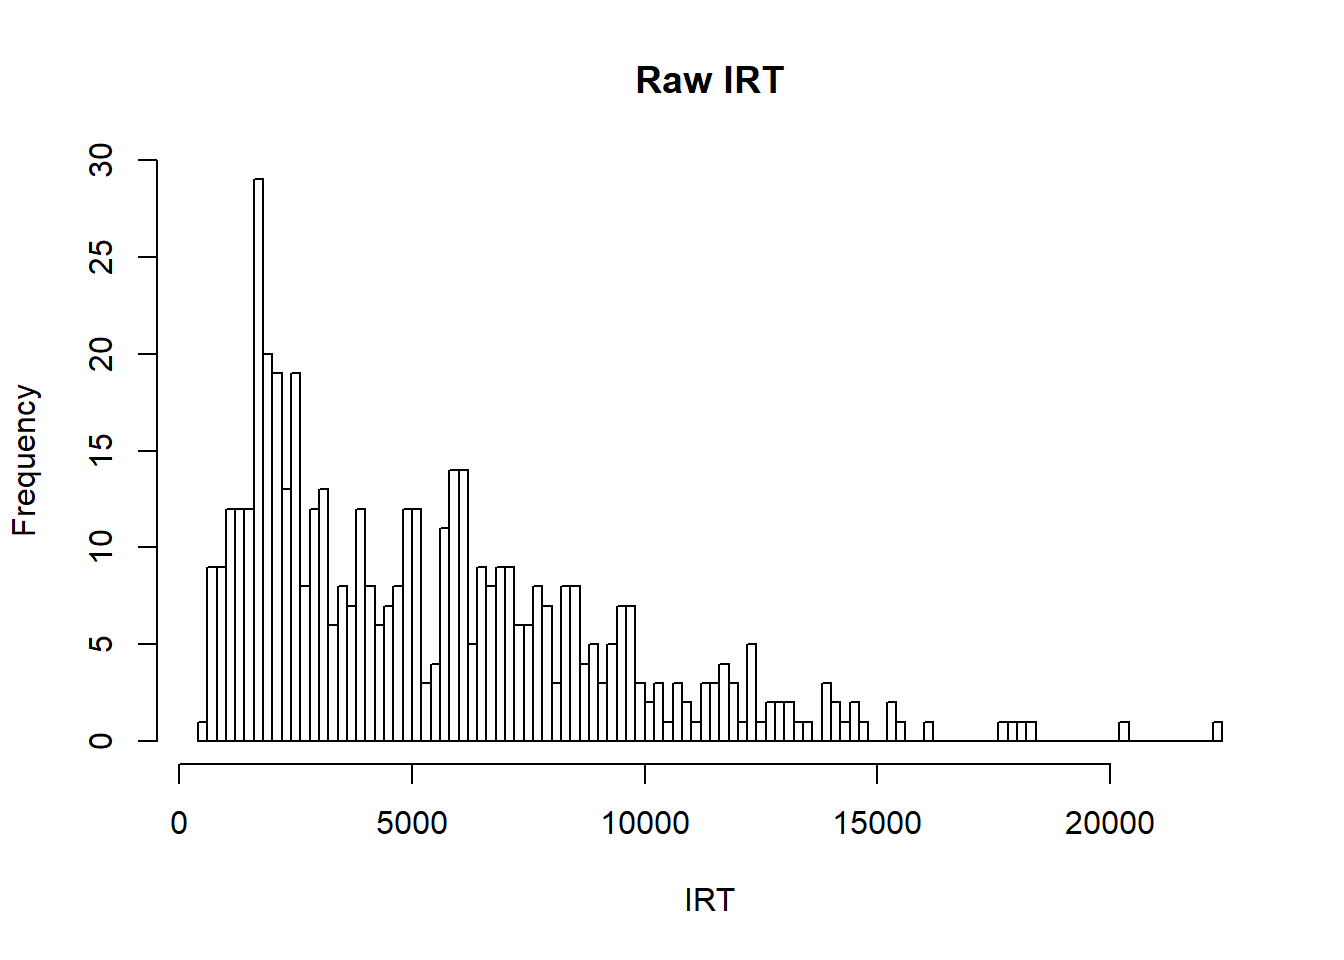
\includegraphics{results_files/figure-latex/rawIRThist-1} \caption[Distribution of raw IRT]{Distribution of raw IRT}\label{fig:rawIRThist}
\end{figure}

IRTs below 250ms (2) and above 25s (5) are (assumed to be implausible)
omitted. Experimental data were then Winsorized by participant to bring
data in the 5th and 95th percentile of data to the value at those
tresholds. The resulting measure is referred to as wIRT and is
distribued as shown in Figure \ref{fig:wIRT} (n = 495). Overall mean for
wIRT is 6.6s. The longest IRT is 22.8s and the shortest is 737ms. Median
wIRT is 6.1s.

\begin{figure}
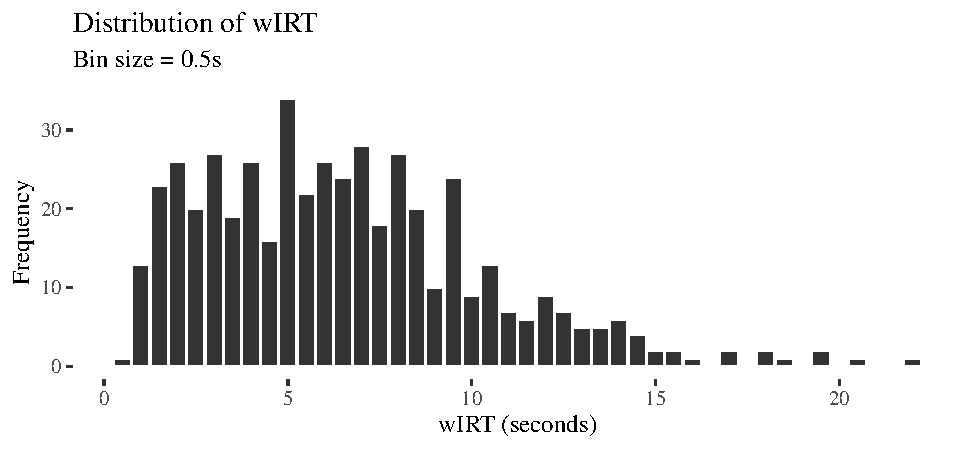
\includegraphics{results_files/figure-latex/wIRT-1} \caption[Distribution of wIRT]{Distribution of wIRT}\label{fig:wIRT}
\end{figure}

For the purposes of regression analysis, a common log transformation
reduces the skew in the data. This distribution is seen in Figure
\ref{fig:log10wins}.

\begin{figure}
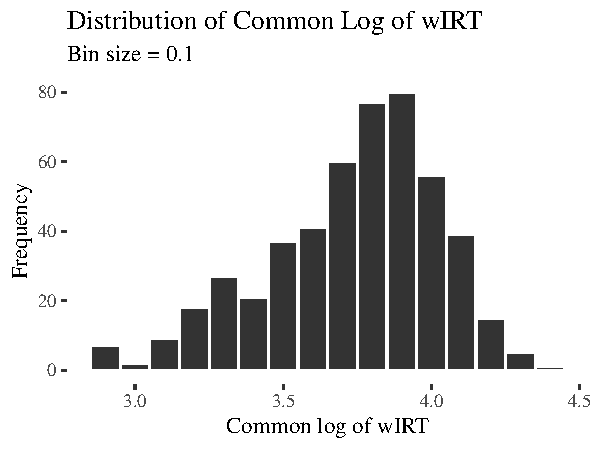
\includegraphics{results_files/figure-latex/log10wins-1} \caption[Common log of wIRT]{Common log of wIRT}\label{fig:log10wins}
\end{figure}

\section{Means by condition}\label{means-by-condition}

Table \ref{tab:mns} shows the mean wIRT by experimental condition. The
top left cell represents the mean wIRT for the declaritive controls
(``-Q -GP''). The bottom row shows the increase in IRT across the garden
path condition.

\begin{table}[t]

\caption{\label{tab:mns}Means (s) by condition}
\centering
\begin{tabular}{lrr}
\toprule
Condition & -Q & +Q\\
\midrule
-GP & 6.20 & 6.56\\
+GP & 6.67 & 6.94\\
Increase & 0.47 & 0.39\\
\bottomrule
\end{tabular}
\end{table}

The difference in the effect of ±GP across ±Q is 82ms. This difference
is in the direction that supports the hypothesis.

\begin{figure}
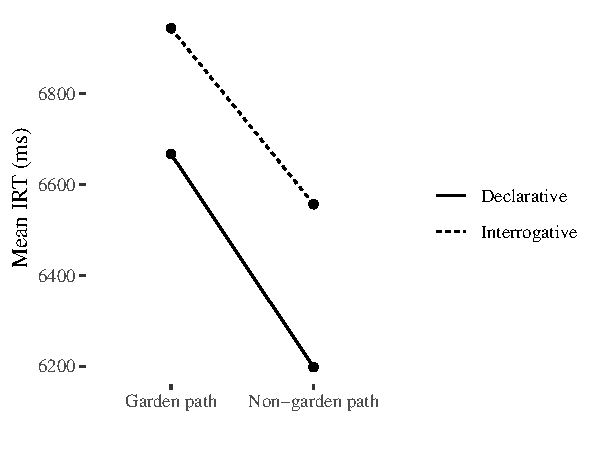
\includegraphics{results_files/figure-latex/interactinplot-1} \caption[Mean IRT by condition]{Mean IRT by condition}\label{fig:interactinplot}
\end{figure}

\section{Regression models}\label{regression-models}

The models with random slopes for participant and item did not converge,
so the tables in this section show models with no random slopes.

For the first model, fixed effects of ±GP and ±Q as well is the
interaction between them were included, along with random effects of
participant and item. The second model removes the interaction, but
keeps both main effects.

\begin{table}[!htbp] \centering 
  \caption{Interaction vs. non-interaction model} 
  \label{} 
\begin{tabular}{@{\extracolsep{5pt}}lcc} 
\\[-1.8ex]\hline 
\hline \\[-1.8ex] 
 & \multicolumn{2}{c}{\textit{Dependent variable:}} \\ 
\cline{2-3} 
\\[-1.8ex] & \multicolumn{2}{c}{Winsorized IRT} \\ 
\\[-1.8ex] & (1) & (2)\\ 
\hline \\[-1.8ex] 
 +GP & 362.077 & 367.485$^{*}$ \\ 
  & (285.543) & (202.990) \\ 
  & & \\ 
 +Q & 458.456 & 463.912$^{**}$ \\ 
  & (286.773) & (202.953) \\ 
  & & \\ 
 +GP +Q & 10.939 &  \\ 
  & (406.230) &  \\ 
  & & \\ 
 Constant & 6,279.529$^{***}$ & 6,276.827$^{***}$ \\ 
  & (595.388) & (586.867) \\ 
  & & \\ 
\hline \\[-1.8ex] 
Observations & 495 & 495 \\ 
Log Likelihood & $-$4,583.130 & $-$4,583.131 \\ 
Akaike Inf. Crit. & 9,180.261 & 9,178.262 \\ 
Bayesian Inf. Crit. & 9,209.693 & 9,203.489 \\ 
\hline 
\hline \\[-1.8ex] 
\textit{Note:}  & \multicolumn{2}{r}{$^{*}$p$<$0.1; $^{**}$p$<$0.05; $^{***}$p$<$0.01} \\ 
\end{tabular} 
\end{table}

A model with no fixed effects was also run, here it is shown beside the
interaction model from the previous table.

\begin{table}[!htbp] \centering 
  \caption{Interaction vs. no fixed effects} 
  \label{} 
\begin{tabular}{@{\extracolsep{5pt}}lcc} 
\\[-1.8ex]\hline 
\hline \\[-1.8ex] 
 & \multicolumn{2}{c}{\textit{Dependent variable:}} \\ 
\cline{2-3} 
\\[-1.8ex] & \multicolumn{2}{c}{Winsorized IRT} \\ 
\\[-1.8ex] & (1) & (2)\\ 
\hline \\[-1.8ex] 
 +GP & 362.077 &  \\ 
  & (285.543) &  \\ 
  & & \\ 
 +Q & 458.456 &  \\ 
  & (286.773) &  \\ 
  & & \\ 
 +GP +Q & 10.939 &  \\ 
  & (406.230) &  \\ 
  & & \\ 
 Constant & 6,279.529$^{***}$ & 6,689.403$^{***}$ \\ 
  & (595.388) & (568.522) \\ 
  & & \\ 
\hline \\[-1.8ex] 
Observations & 495 & 495 \\ 
Log Likelihood & $-$4,583.130 & $-$4,587.332 \\ 
Akaike Inf. Crit. & 9,180.261 & 9,182.664 \\ 
Bayesian Inf. Crit. & 9,209.693 & 9,199.482 \\ 
\hline 
\hline \\[-1.8ex] 
\textit{Note:}  & \multicolumn{2}{r}{$^{*}$p$<$0.1; $^{**}$p$<$0.05; $^{***}$p$<$0.01} \\ 
\end{tabular} 
\end{table}

\begin{table}[!htbp] \centering 
  \caption{Interaction vs. no random effects} 
  \label{} 
\begin{tabular}{@{\extracolsep{5pt}}lcc} 
\\[-1.8ex]\hline 
\hline \\[-1.8ex] 
 & \multicolumn{2}{c}{\textit{Dependent variable:}} \\ 
\cline{2-3} 
\\[-1.8ex] & \multicolumn{2}{c}{Winsorized IRT} \\ 
\\[-1.8ex] & \textit{linear} & \textit{OLS} \\ 
 & \textit{mixed-effects} & \textit{} \\ 
\\[-1.8ex] & (1) & (2)\\ 
\hline \\[-1.8ex] 
 +GP & 362.077 & 358.335 \\ 
  & (285.543) & (487.048) \\ 
  & & \\ 
 +Q & 458.456 & 468.453 \\ 
  & (286.773) & (489.024) \\ 
  & & \\ 
 +GP +Q & 10.939 & $-$81.632 \\ 
  & (406.230) & (692.298) \\ 
  & & \\ 
 Constant & 6,279.529$^{***}$ & 6,198.129$^{***}$ \\ 
  & (595.388) & (344.395) \\ 
  & & \\ 
\hline \\[-1.8ex] 
Observations & 495 & 495 \\ 
R$^{2}$ &  & 0.005 \\ 
Adjusted R$^{2}$ &  & $-$0.001 \\ 
Log Likelihood & $-$4,583.130 &  \\ 
Akaike Inf. Crit. & 9,180.261 &  \\ 
Bayesian Inf. Crit. & 9,209.693 &  \\ 
Residual Std. Error &  & 3,850.452 (df = 491) \\ 
F Statistic &  & 0.793 (df = 3; 491) \\ 
\hline 
\hline \\[-1.8ex] 
\textit{Note:}  & \multicolumn{2}{r}{$^{*}$p$<$0.1; $^{**}$p$<$0.05; $^{***}$p$<$0.01} \\ 
\end{tabular} 
\end{table}

\section{Delay comparison for cold vs.~previewed
readings}\label{delay-comparison-for-cold-vs.previewed-readings}

A comparison of the delay for cold readings compared with that of
previewed readings can lend insight into the extent to which subjects
followed task instructions.

``Delay'' here is the amount of time after the start of a recording
until the beginning of phonation of the target sentence. Cold readings
are also called ``reading 1'', while previewed readings are the same as
``reading 2''. Implausible delays of \textgreater{}15s are excluded in
the data shown here.

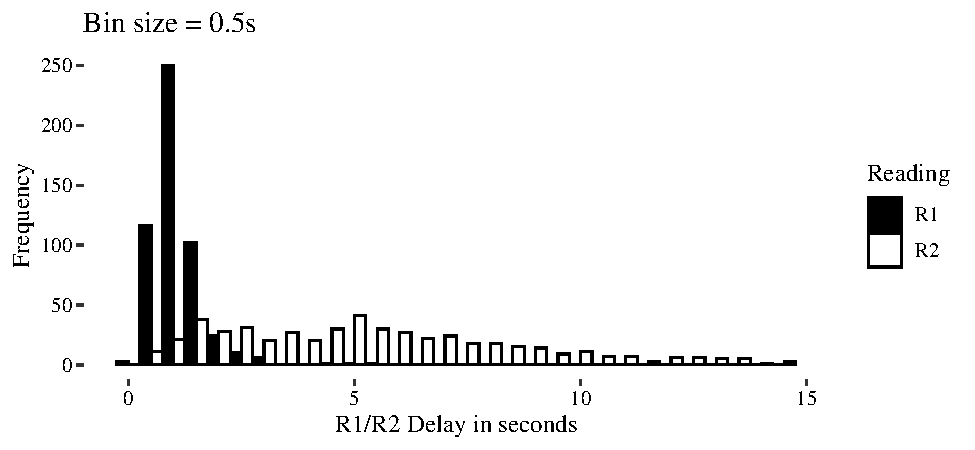
\includegraphics{results_files/figure-latex/delayComparison-1}

For cold readings, n = 514 and for previewed, n = 497.

\subsection{Difference in delay across paired
readings}\label{difference-in-delay-across-paired-readings}

Overall, each recording pair (n = 497) has a mean difference in delay
(DelDif = previewed delay - cold delay) of 4.3s (sd = 3.3s), with a
minumum of -1.9s and a max of 13.4s. The median DelDif is 3.9s. The
distribution DelDif is shown in Figure \ref{fig:deddif}.

\begin{figure}
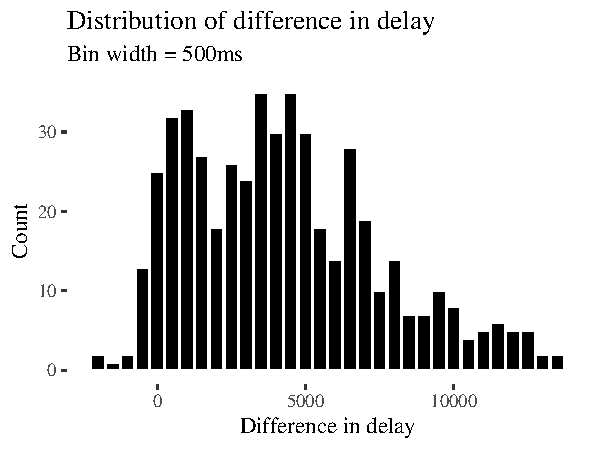
\includegraphics{results_files/figure-latex/deddif-1} \caption[Distribution of DelDif]{Distribution of DelDif}\label{fig:deddif}
\end{figure}

If we calculate the mean delay difference by participant, we find a mean
participant DelDef of 4.4s. Each participant's DelDif is ≤ 386ms and ≥
10.2s, with a median of 3.97s. Table \ref{tab:difsbyp} shows these
values.

\begin{longtable}{lrr}
\caption{\label{tab:difsbyp}Delay differences by participant}\\
\toprule
  & Participant & Mean difference in delay (ms)\\
\midrule
1 & 1 & 386\\
8 & 8 & 702\\
23 & 203 & 938\\
28 & 208 & 1183\\
29 & 209 & 1290\\
\addlinespace
24 & 204 & 1502\\
22 & 201 & 1584\\
32 & 214 & 1604\\
26 & 206 & 2582\\
33 & 215 & 2814\\
\addlinespace
20 & 21 & 2908\\
17 & 17 & 3139\\
31 & 212 & 3167\\
7 & 7 & 3682\\
9 & 9 & 3816\\
\addlinespace
30 & 210 & 3908\\
21 & 22 & 3973\\
27 & 207 & 3988\\
12 & 12 & 4303\\
2 & 2 & 4369\\
\addlinespace
4 & 4 & 4798\\
3 & 3 & 4841\\
11 & 11 & 4845\\
15 & 15 & 5961\\
10 & 10 & 6358\\
\addlinespace
25 & 205 & 6858\\
14 & 14 & 7157\\
5 & 5 & 7838\\
13 & 13 & 8051\\
19 & 20 & 8685\\
\addlinespace
16 & 16 & 9105\\
18 & 19 & 9537\\
6 & 6 & 10184\\
\bottomrule
\end{longtable}

The distribution of the participants' DelDifs can be found in Figure
\ref{fig:difhistbyp}.

\begin{figure}
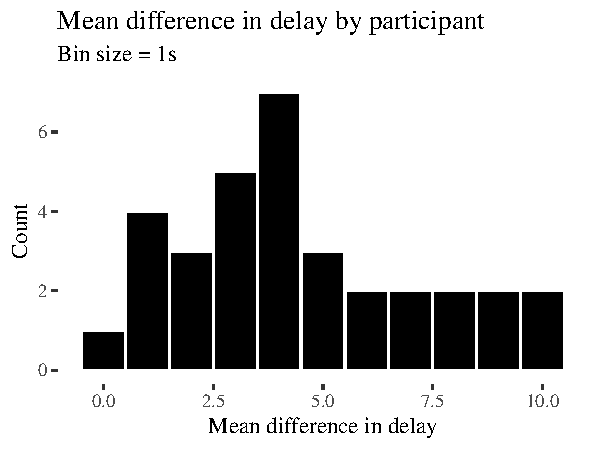
\includegraphics{results_files/figure-latex/difhistbyp-1} \caption[Mean difference in delay by participant]{Mean difference in delay by participant}\label{fig:difhistbyp}
\end{figure}

\section{Individual variation}\label{individual-variation}

Individuals vary with regard to the effect of the garden path condition
on IRT. For 18 of 32, the increase in IRT for garden paths is greater
for interrogatives than it is for declaratives.

\begin{longtable}{lrrrr}
\caption{\label{tab:pPattern}Mean wIRT (ms) by condition and participant}\\
\toprule
Participant & -Q -GP & -Q +GP & +Q -GP & +Q +GP\\
\midrule
12 & 5436.092 & 5236.717 & 6146.935 & 7347.062\\
17 & 3725.878 & 6283.250 & 5736.560 & 5128.127\\
1 & 2723.095 & 2764.875 & 3165.468 & 3061.438\\
10 & 9072.500 & 9416.155 & 8734.438 & 9630.157\\
11 & 8635.833 & 9030.440 & 5688.040 & 12075.837\\
\addlinespace
13 & 10779.875 & 11638.595 & 9410.875 & 11132.593\\
14 & 7180.315 & 8851.722 & 8443.062 & 12052.435\\
15 & 9673.310 & 7771.158 & 9463.500 & 5764.438\\
16 & 12583.907 & 9725.440 & 9352.470 & 15201.440\\
19 & 8780.500 & 14237.875 & 17076.783 & 16161.185\\
\addlinespace
2 & 6077.595 & 7088.435 & 4410.845 & 6398.435\\
20 & 9963.565 & 9211.125 & 12225.282 & 10081.030\\
201 & 1396.033 & 4249.562 & 2533.628 & 2206.812\\
203 & 1451.470 & 1501.438 & 1909.753 & 2472.343\\
204 & 3164.688 & 3173.847 & 2792.125 & 1676.000\\
\addlinespace
205 & 6456.967 & 11925.468 & 7450.278 & 11345.407\\
206 & 3736.810 & 3707.875 & 3223.593 & 4985.440\\
207 & 5083.280 & 6428.315 & 6700.748 & 5199.312\\
208 & 2612.250 & 3449.810 & 2482.940 & 3263.970\\
209 & 2126.185 & 3625.500 & 2563.718 & 2967.907\\
\addlinespace
21 & 5035.065 & 5748.627 & 6117.688 & 7204.748\\
210 & 5690.440 & 6105.592 & 6664.688 & 5098.160\\
212 & 4699.658 & 5192.250 & 4647.190 & 5065.035\\
214 & 3628.378 & 4118.707 & 5185.467 & 2026.030\\
215 & 4432.130 & 4132.312 & 5207.998 & 5075.938\\
\addlinespace
22 & 5066.752 & 4134.533 & 5006.845 & 7975.283\\
3 & 5655.472 & 8400.845 & 6056.405 & 7267.347\\
4 & 7993.717 & 5457.905 & 10609.750 & 7010.720\\
5 & 13082.620 & 10694.565 & 9437.685 & 12188.125\\
6 & 12848.093 & 10828.407 & 13018.030 & 14695.872\\
\addlinespace
7 & 5208.465 & 5864.283 & 6291.778 & 4918.595\\
9 & 6234.815 & 6632.685 & 6386.938 & 6484.312\\
\bottomrule
\end{longtable}

\begin{figure}
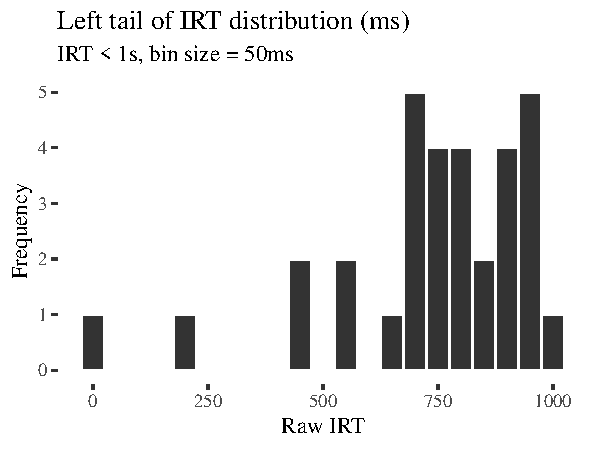
\includegraphics{results_files/figure-latex/irtzoomLft-1} \caption[Left tail of raw IRT distribution]{Left tail of raw IRT distribution}\label{fig:irtzoomLft}
\end{figure}

\begin{figure}
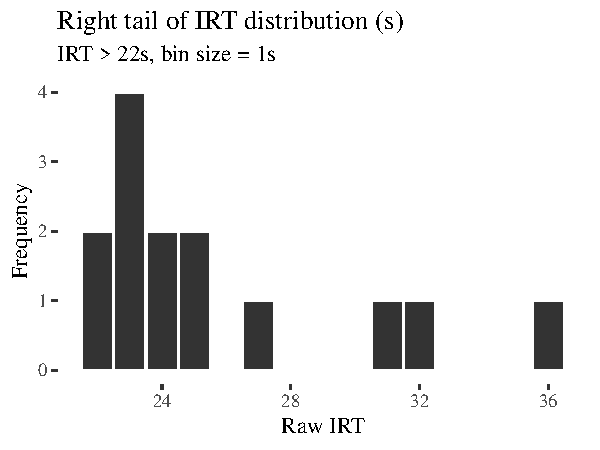
\includegraphics{results_files/figure-latex/zoomRgt-1} \caption[Right tail of raw IRT distribution]{Right tail of raw IRT distribution}\label{fig:zoomRgt}
\end{figure}

\hypertarget{refs}{}
\hypertarget{ref-gmm1}{}
Falk, Tiago H., and Wai-Yip Chan. 2006. ``Nonintrusive Speech Quality
Estimation Using Gaussian Mixture Models.'' \emph{IEEE Signal Processing
Letters} 13 (2). IEEE: 108--11.



\end{document}
